% ----------------------------------------------------------------------------
% O básico de um external
% ----------------------------------------------------------------------------

\chapter{O básico de um external}

Escrever um external significa seguir as recomendações da API. Peço ao leitor
bastante paciência pois este tutorial pretende andar um pouco devagar para
mostrar os passos da escrita de um external.

\section{Meu primeiro external}

Um external necessita de uma estrutura de dados como uma classe em C. Esta
estutura deverá obrigatoriamente possuir um atributo do tipo t\_object. Outros
atributos podem ser adicionados nesta estrutura de maneira que cada instância
da mesma possua os dados necessários para sua execução. Um objeto contador,
por exemplo, pode constar o contador e um objeto que abra um arquivo pode
possuir o caminho do arquivo. O básico desta estrutura é mostrado abaixo.

\begin{lstlisting}

static t_class *example1_class;

typedef struct _example1 {
    t_object x_obj;
} t_example1;
\end{lstlisting}

Todo external deve ter um método com o nome do próprio arquivo + \_setup().
Assim, o puredata irá procurar no arquivo trigger.pd\_linux o método
trigger\_setup(void) e no arquivo osc$\sim$.pd\_linux o método
osc\_tilde\_setup(void). Independente de o mesmo ser um único external ou uma
biblioteca. Veja que objetos que recebem áudio e que, por consequência possuem
$\sim$ no seu nome, possuem \_tilde\_setup na assinatura de seu método. É do
método setup() que começamos tudo.

\begin{lstlisting}

void example1_setup(void) {
    example1_class = class_new(gensym("example1"),
            (t_newmethod) example1_new, // Constructor
            0,
            sizeof (t_example1),
	    CLASS_NOINLET,
            0);
}
\end{lstlisting}

Na chamada do método setup() podemos ter a construção de um objeto (Veja o
exemplo 01) ou uma biblioteca com vários objetos (Veja exemplo 03). A
construção de um objeto é feita a partir da função class\_new(). Esta função
recebe vários parâmetros como:

\begin{itemize}
\item nome do objeto
\item função construtora do objeto
\item função destrutora do objeto
\item tamanho do objeto
\item Tipo da classe do objeto
\item Parâmetros a serem passados para o objeto na sua construção (Podem ser vários - Veja o próximo capítulo)
\item Zero.
\end{itemize}

É obrigatório que o último parâmetro seja 0 pois isto indicará ao PD que os
parâmetros terminaram.

O tipo da classe pode definir seu comportamento. Estes tipos são:

\begin{itemize}
\item CLASS\_DEFAULT 0
\item CLASS\_PD 1
\item CLASS\_GOBJ 2
\item CLASS\_PATCHABLE 3
\item CLASS\_NOINLET 8
\end{itemize}

(Retirado do arquivo m\_pd.h)

*** Usei apenas o 0 e o 8. Experimentarei usar os outros tipos.

A função class\_new() será utilizada para construir o objeto. Nesta função,
além de criarmos o novo objeto com a função pd\_new, podemos definir os
valores dos atributos da nossa estrutura de dados e inicializar qualquer
contexto que seja necessário, como abrir arquivos, popular arrays e outras
coisas.

\begin{lstlisting}
// Constructos of the class
void * example1_new(void) {
    t_example1 *x = (t_example1 *) pd_new(example1_class);
    return (void *) x;
}
\end{lstlisting}

Se tudo foi feito corretamente, compilado e colocado no PD, temos o resultado.

\begin{figure}[h!]
	\centering
	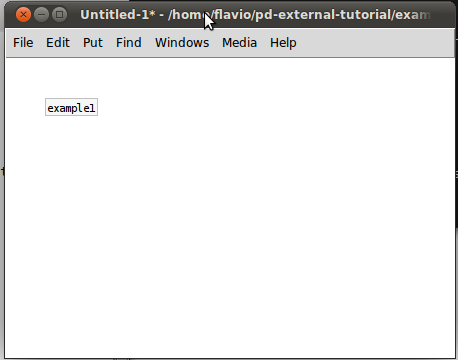
\includegraphics[width=0.7\textwidth]{example1}
	\caption{Nosso primeiro external do PD. Ainda inútil.:-)}
\end{figure}

\section{Minha primeira biblioteca}

Um mesmo método setup pode definir vários objetos de classes diferentes. A
isto damos o nome de biblioteca. Para isto, o método setup() terá o mesmo nome
do arquivo com a biblioteca mas os objetos podem ter outros nomes. Veja o
exemplo03.

\begin{lstlisting}

void example3_setup(void) {
    post("Initializing my library");

    myobj1_class = class_new(gensym("myobj1"),
            (t_newmethod) myobj1_new, // Constructor
            0,
            sizeof (t_myobj1),
	    CLASS_NOINLET,
            0);
    class_sethelpsymbol(myobj1_class, 
	gensym("myobj1-help"));

    myobj2_class = class_new(gensym("myobj2"),
            (t_newmethod) myobj2_new, // Constructor
            0,
            sizeof (t_myobj2),
	    CLASS_NOINLET,
            0);
    class_sethelpsymbol(myobj2_class, 
	gensym("myobj2-help"));

}
\end{lstlisting}

Se o arquivo foi feito corretamente, compilado corretamente e adicionado ao
caminho do PureData, teremos o resultado.

\begin{figure}[h!]
	\centering
	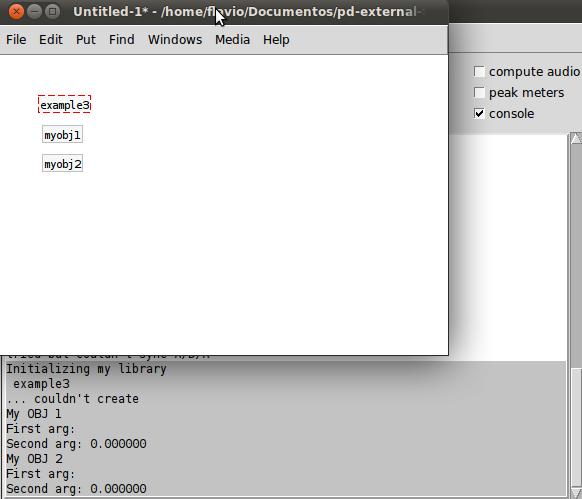
\includegraphics[width=0.7\textwidth]{example3}
	\caption{Nosso primeiro external do PD. Ainda inútil.:-)}
\end{figure}


No caso da biblioteca, podemos ter um arquivo de help para cada external. Esta
associação é feita pela função:

\begin{lstlisting}
class_sethelpsymbol(myclass_class, gensym("my_class-help"));
\end{lstlisting}

Um objeto pode ainda ter outros nomes ou alias. Para definir isto podemo utilizar a função class\_addcreator. Veja o exemplo:

\begin{lstlisting}
class_addcreator((t_newmethod)medusa_new, gensym("med"), 0);
\end{lstlisting}

\section{Variáveis globais}

Você pode usar uma variável global para armazenar dados pelos seus externals.
Esta variável será visível para todas as intâncias do external e todas podem
alterar seu valor. Isto pode ser útil ou um desastre. (Veja o exemplo16).

\begin{lstlisting}
int count = 0;

void * example16_new(void) {
    t_example16 *x = (t_example16 *) pd_new(example16_class);
    post("Counter value: %d",count);
    count++;
    return (void *) x;
}
\end{lstlisting}

\begin{figure}[h!]
	\centering
	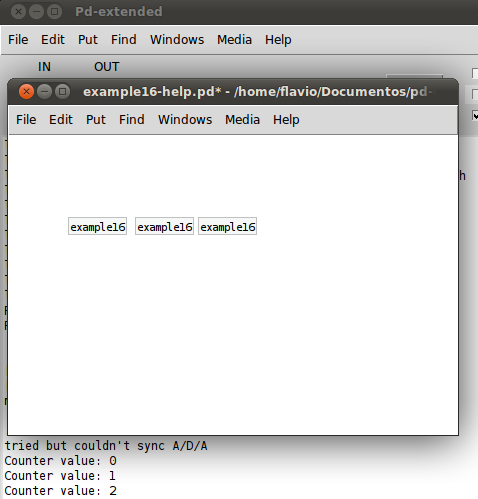
\includegraphics[width=0.7\textwidth]{example16}
	\caption{Repare no output da janela principal.}
\end{figure}

Caso isto não seja desejável, o ideal é colocar suas variáveis dentro da
struct do objeto. Assim cada instância terá seu próprio contador.

\begin{lstlisting}

static t_class *example_class;

typedef struct _example {
    t_object x_obj;
    t_int counter;
} t_example;

void * example_new(void) {
    t_example *x = (t_example *) pd_new(example_class);
    post("Counter value: %d",x->counter);
    counter++;
    return (void *) x;
}

\end{lstlisting}

